% (The MIT License)
%
% Copyright (c) 2023-2024 Yegor Bugayenko
%
% Permission is hereby granted, free of charge, to any person obtaining a copy
% of this software and associated documentation files (the 'Software'), to deal
% in the Software without restriction, including without limitation the rights
% to use, copy, modify, merge, publish, distribute, sublicense, and/or sell
% copies of the Software, and to permit persons to whom the Software is
% furnished to do so, subject to the following conditions:
%
% The above copyright notice and this permission notice shall be included in all
% copies or substantial portions of the Software.
%
% THE SOFTWARE IS PROVIDED 'AS IS', WITHOUT WARRANTY OF ANY KIND, EXPRESS OR
% IMPLIED, INCLUDING BUT NOT LIMITED TO THE WARRANTIES OF MERCHANTABILITY,
% FITNESS FOR A PARTICULAR PURPOSE AND NONINFRINGEMENT. IN NO EVENT SHALL THE
% AUTHORS OR COPYRIGHT HOLDERS BE LIABLE FOR ANY CLAIM, DAMAGES OR OTHER
% LIABILITY, WHETHER IN AN ACTION OF CONTRACT, TORT OR OTHERWISE, ARISING FROM,
% OUT OF OR IN CONNECTION WITH THE SOFTWARE OR THE USE OR OTHER DEALINGS IN THE
% SOFTWARE.

\documentclass{article}
\usepackage{../lecture-notes/notes}
\usepackage{setspace}
\newcommand*\thetitle{TCC and LCC}
\begin{document}

\plush{\lnTitlePage{8}{24}{JOKxjpAglFU}}

\lnQuote
  {socrates}
  {\textbf{Socrates}: I am a lover of these processes of \ul{division} and \ul{bringing together}, as aids to speech and thought; and if I think any other man is able to see things that can naturally be collected into one and divided into many, him I follow after and walk in his footsteps as if he were a god.}
  {plato370}

\lnQuote
  [Edward Yourdon]
  {edward-yourdon}
  {Module cohesion may be conceptualized as the \ul{cement} that holds the processing elements of a module together. In a sense, a high degree of module cohesion is an indication of \ul{close approximation} of inherent problem structure.}
  {yourdon1979structured}

\lnQuote
  [Andrew Hunt]
  {andy-hunt}
  {We want to design components that are self-contained: independent, and with a \ul{single}, well-defined purpose.}
  {hunt1999pragmatic}

\lnQuote
  [James M. Bieman]
  {james-bieman}
  {We define two measures of class cohesion based on the \ul{direct} and \ul{indirect} connections of method pairs: TCC and LCC.}
  {bieman1995cohesion}

\pptBanner{Tight and Loose Class Cohesion (TCC+LCC)}
\begin{multicols}{2}
{\small\begin{ffcode}
class Rectangle
  int x, y, w, h;
  int area()
    return w * h;
  int move(int dx, dy)
    x += dx; y += dy;
  int resize(int dx, dy)
    w += dx; h += dy;
  bool fit()
    return w < 100
      && x < 100;
\end{ffcode}
}
\par\columnbreak\par
Max possible connections (\texttt{NP}): \\
\( N \times (N-1) / 2 = 4 \times 3 / 2 = 6\)
\par
Directly connected (\(\texttt{NDC}=4\)): \\
\texttt{area+fit}, \texttt{area+resize}, \texttt{move+fit}, \texttt{resize+fit}
\par
Indirectly connected (\(\texttt{NIC}=2\)): \\
\texttt{area+move}, \texttt{move+resize}
\par
\(\texttt{TCC} = \texttt{NDC} / \texttt{NP} = 4/6 = 0.66 \) \\
\(\texttt{LCC} = (\texttt{NDC} + \texttt{NIC}) / \texttt{NP} = 6/6 = 1.00 \) \\
\end{multicols}
\plush{}

\lnQuote
  {../08-TCC-and-LCC/paper}
  {If a class is designed in \ul{ad hoc manner} and unrelated components are included in the class, the class represents more than one concept and does not \ul{model an entity}. The cohesion value of such a class is likely to be less than 0.5.}
  {bieman1995cohesion}

\lnQuote
  [Steve McConnell]
  {steve-mcconnell}
  {Cohesion refers to how closely all the routines in a class or all the code in a routine support a \ul{central purpose}---how focused the class is. The ideas of \ul{abstraction} and cohesion are closely related---a class interface that presents a good abstraction usually has strong cohesion.}
  {mcconnell2004code}

\pptBanner{Abstraction}
\begin{multicols}{2}
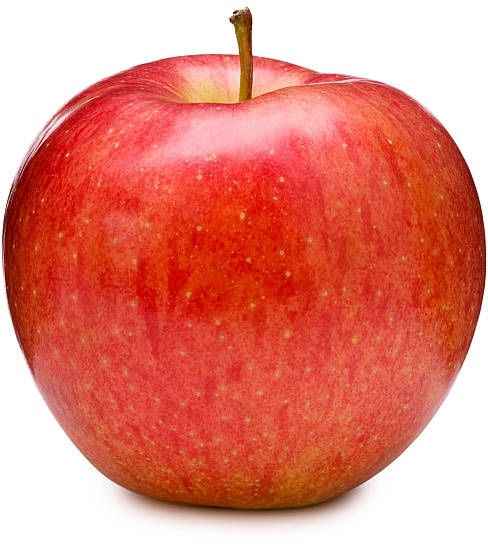
\includegraphics[width=1.3in]{apple.jpg}
\begin{itemize}\setlength\itemsep{0em}
\item Color: red
\item Weight: 120g
\item Price: \$0.99
\end{itemize}
\par\columnbreak\par

\includegraphics[width=0.8in]{file-on-disc.jpg}
\par
{\small\begin{ffcode}
var file = {
  path: '/tmp/data.txt',
  read: function() { ... },
  write: function(txt) { ... }
}
\end{ffcode}
}
\end{multicols}
\par
{\scriptsize The slide is taken from the \href{https://github.com/yegor256/painofoop}{``Pain of OOP''} (2023) course.\par}
\plush{}

\pptBanner{Inheritance vs. Cohesion}
\begin{multicols}{2}
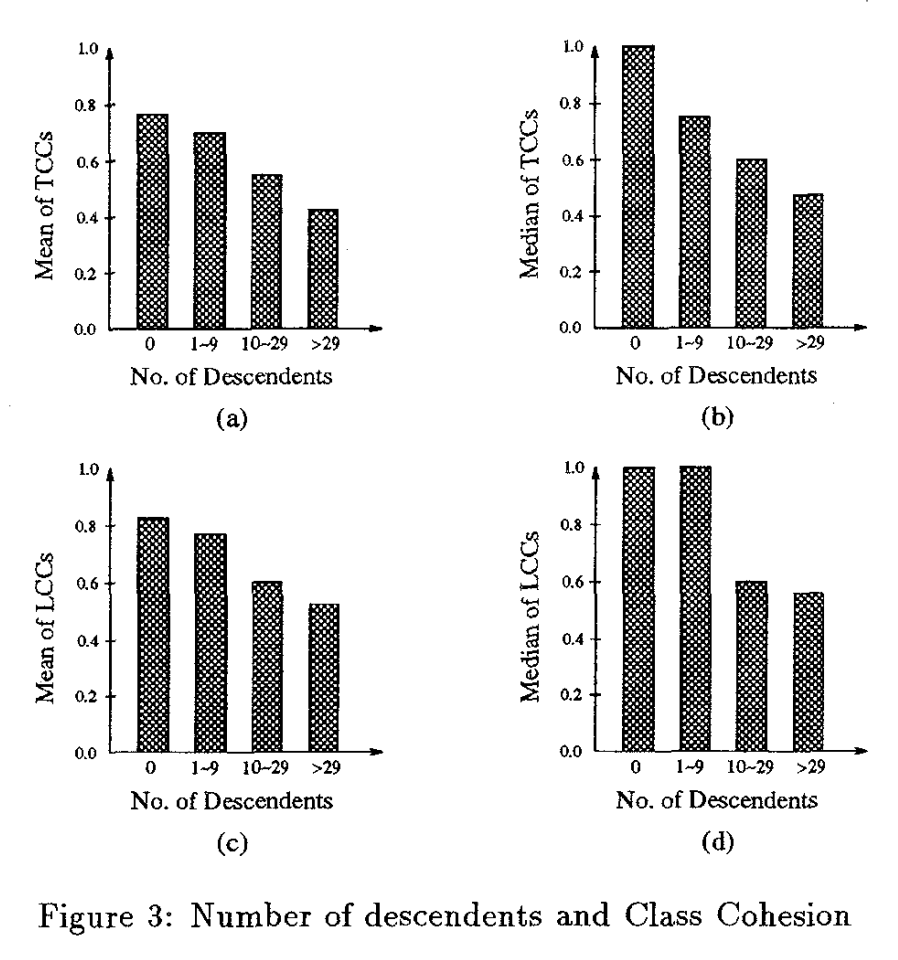
\includegraphics[width=.9\columnwidth]{graphs.png}
\par\columnbreak\par
``Our results show that the classes that are heavily \ul{reused} via inheritance exhibit \ul{lower cohesion}. We expected to find that the most reused classes would be the most cohesive ones.''\par
\lnSource{bieman1995cohesion}
\end{multicols}
\plush{}

\pptBanner{Inheritance is Code Reuse}
\begin{multicols}{2}
{\small\begin{ffcode}
class Manuscript {
  protected String body;
  void print(Console console) {
    console.println(this.body);
  }
}
class Article
  extends Manuscript {
  void submit(Conference cnf) {
    cnf.send(this.body);
  }
}
\end{ffcode}
}
\par\columnbreak\par
\begin{spacing}{0.9}
``The \ff{Article} copies method \ff{print()} and attribute body from the \ff{Manuscript}, as if it’s not a living organism, but rather a dead one from which we \ul{inherit} its parts.''\par
``Implementation inheritance was created as a mechanism for code reuse. It doesn't fit into OOP at all.''\par
\lnSource{bugayenko2016blog0913}
\end{spacing}
\end{multicols}
\plush{}

\pptBanner{Composition over Inheritance}
\begin{multicols}{2}
{\small\begin{ffcode}
class Manuscript
  protected String body;
  void print(Console console)
    console.println(this.body);

class Article
  extends Manuscript
  void submit(Conference cnf)
    cnf.send(this.body);
\end{ffcode}
}
\par\columnbreak\par
{\small\begin{ffcode}
class Manuscript
  protected String body;
  void print(Console console)
    console.println(this.body);

class Article
  Manuscript manuscript;
  Article(Manuscript m)
    this.manuscript = m;
  void submit(Conference cnf)
    cnf.send(this.body);
\end{ffcode}
}
\end{multicols}\par
{\scriptsize Wikipedia: \url{https://en.wikipedia.org/wiki/Composition_over_inheritance}\par}
\plush{}

\lnPitch{TCC+LCC can be calculated by a few tools:
\begin{itemize}
\item \href{https://www.jpeek.org}{jPeek} for Java
\item C++ --- don't know
\item Python --- don't know
\item JavaScript --- don't know
\item C\# --- don't know
\end{itemize}}

\end{document}
